%\section*{\lbtitle Определение интенсивности транспирации весовым методом}
%\addcontentsline{toc}{section}{Определение интенсивности транспирации весовым методом}

%\subsection*{Теоретические положения}

%\paragraph{}\efbox[margin=10pt,backgroundcolor=yellow]{
%	\begin{minipage}{0.95\textwidth}
%	Интенсивность транспирации — это величина, показывающая количество воды испаряющейся с единицы поверхности листа за единицу времени. 
%	\end{minipage}
%	}
	
%\paragraph{}\hyperlink{transpiration_intensivity}{Данная величина} зависит от ряда внешних факторов, таких, как \hyperlink{transpiration_time}{времени суток}, температура, \hyperlink{transpiration_air_humidity}{относительная влажность воздуха} и обычно колеблется в пределах 15-250 г/(м$^2$*ч).

%\paragraph*{}Для определения интенсивности транспирации чаще всего используется весовой метод, который основан на учете потери растением воды при испарении. Весовым методом можно изучать как транспирацию целого растения, так и отдельных его частей. Так как определить интенсивности транспирации у целого растения довольно сложно, чаще всего измерения проводят на срезанных побегах и листьях. Чтобы во время опыта оводненность тканей не снижалась, срезанный лист помещают в прибор Веска, заполненный водой (рисунок \ref{veska}).

%\paragraph*{}Транспирация это физиологически активный процесс и растения способны в некоторых пределах регулировать его интенсивность. Способность растений к регуляции интенсивности транспирации характеризует такой показатель как \textit{относительная транспирация}. 

%\paragraph{}\efbox[margin=10pt,backgroundcolor=yellow]{
%	\begin{minipage}{0.95\textwidth}
%	Относительная транспирация — это отношение интенсивности транспирации к интенсивности испарения со свободной водной поверхности при тех же условиях. 
%	\end{minipage}
%	}	
	
%\paragraph{}Относительная транспирация обычно составляет 0,1-0,5.

\begin{footnotesize}

\paragraph*{}\textbf{Цель работы}: Определить весовым методом \hypertarget{lab_transp_level}{интенсивность} \hyperlink{transpiration}{транспирации} у подсолнечника;

\paragraph*{}\textbf{Оборудование}: Трехнедельные растения подсолнечника, аналитические весы, часы, прибор Веска, чашки Петри, ножницы, бумага, линейка, вата;

\end{footnotesize}

\subsection*{Ход работы}

\subsubsection*{Подготовка прибора Веска}

\paragraph*{}Со стебля используемого для опыта растения, срежьте лист вместе с черешком. Черешок срезанного листа поместите в отверстие резиновой пробки прибора Веска и  плотно укрепите там ватой. 

\paragraph*{\warningsign}Следует помнить, что конец черешка должен выступать из нижней части пробки настолько, чтобы в собранном приборе он был погружен в воду. 

\paragraph*{}Нижний конец черешка подрезается наискось под водой примерно на 1 см. Эта операция необходима для восстановления водяных нитей в проводящих сосудах. Пробка с укрепленным на ней листом вставляется в прибор Веска, наполненный водой комнатной температуры (рисунок \ref{veska}).  

%%%%%%%%%%%%%%%%%%%%%%%%%%%%%%%%%%%%%%%%%%%%%%%%%%%%%%%%%%%%%%%%%%%%%%%%%%%%%%%%%%%%%%%%%%%%%%%%%%%%%%%%%%% 
\begin{figure}[h]
  \centering
       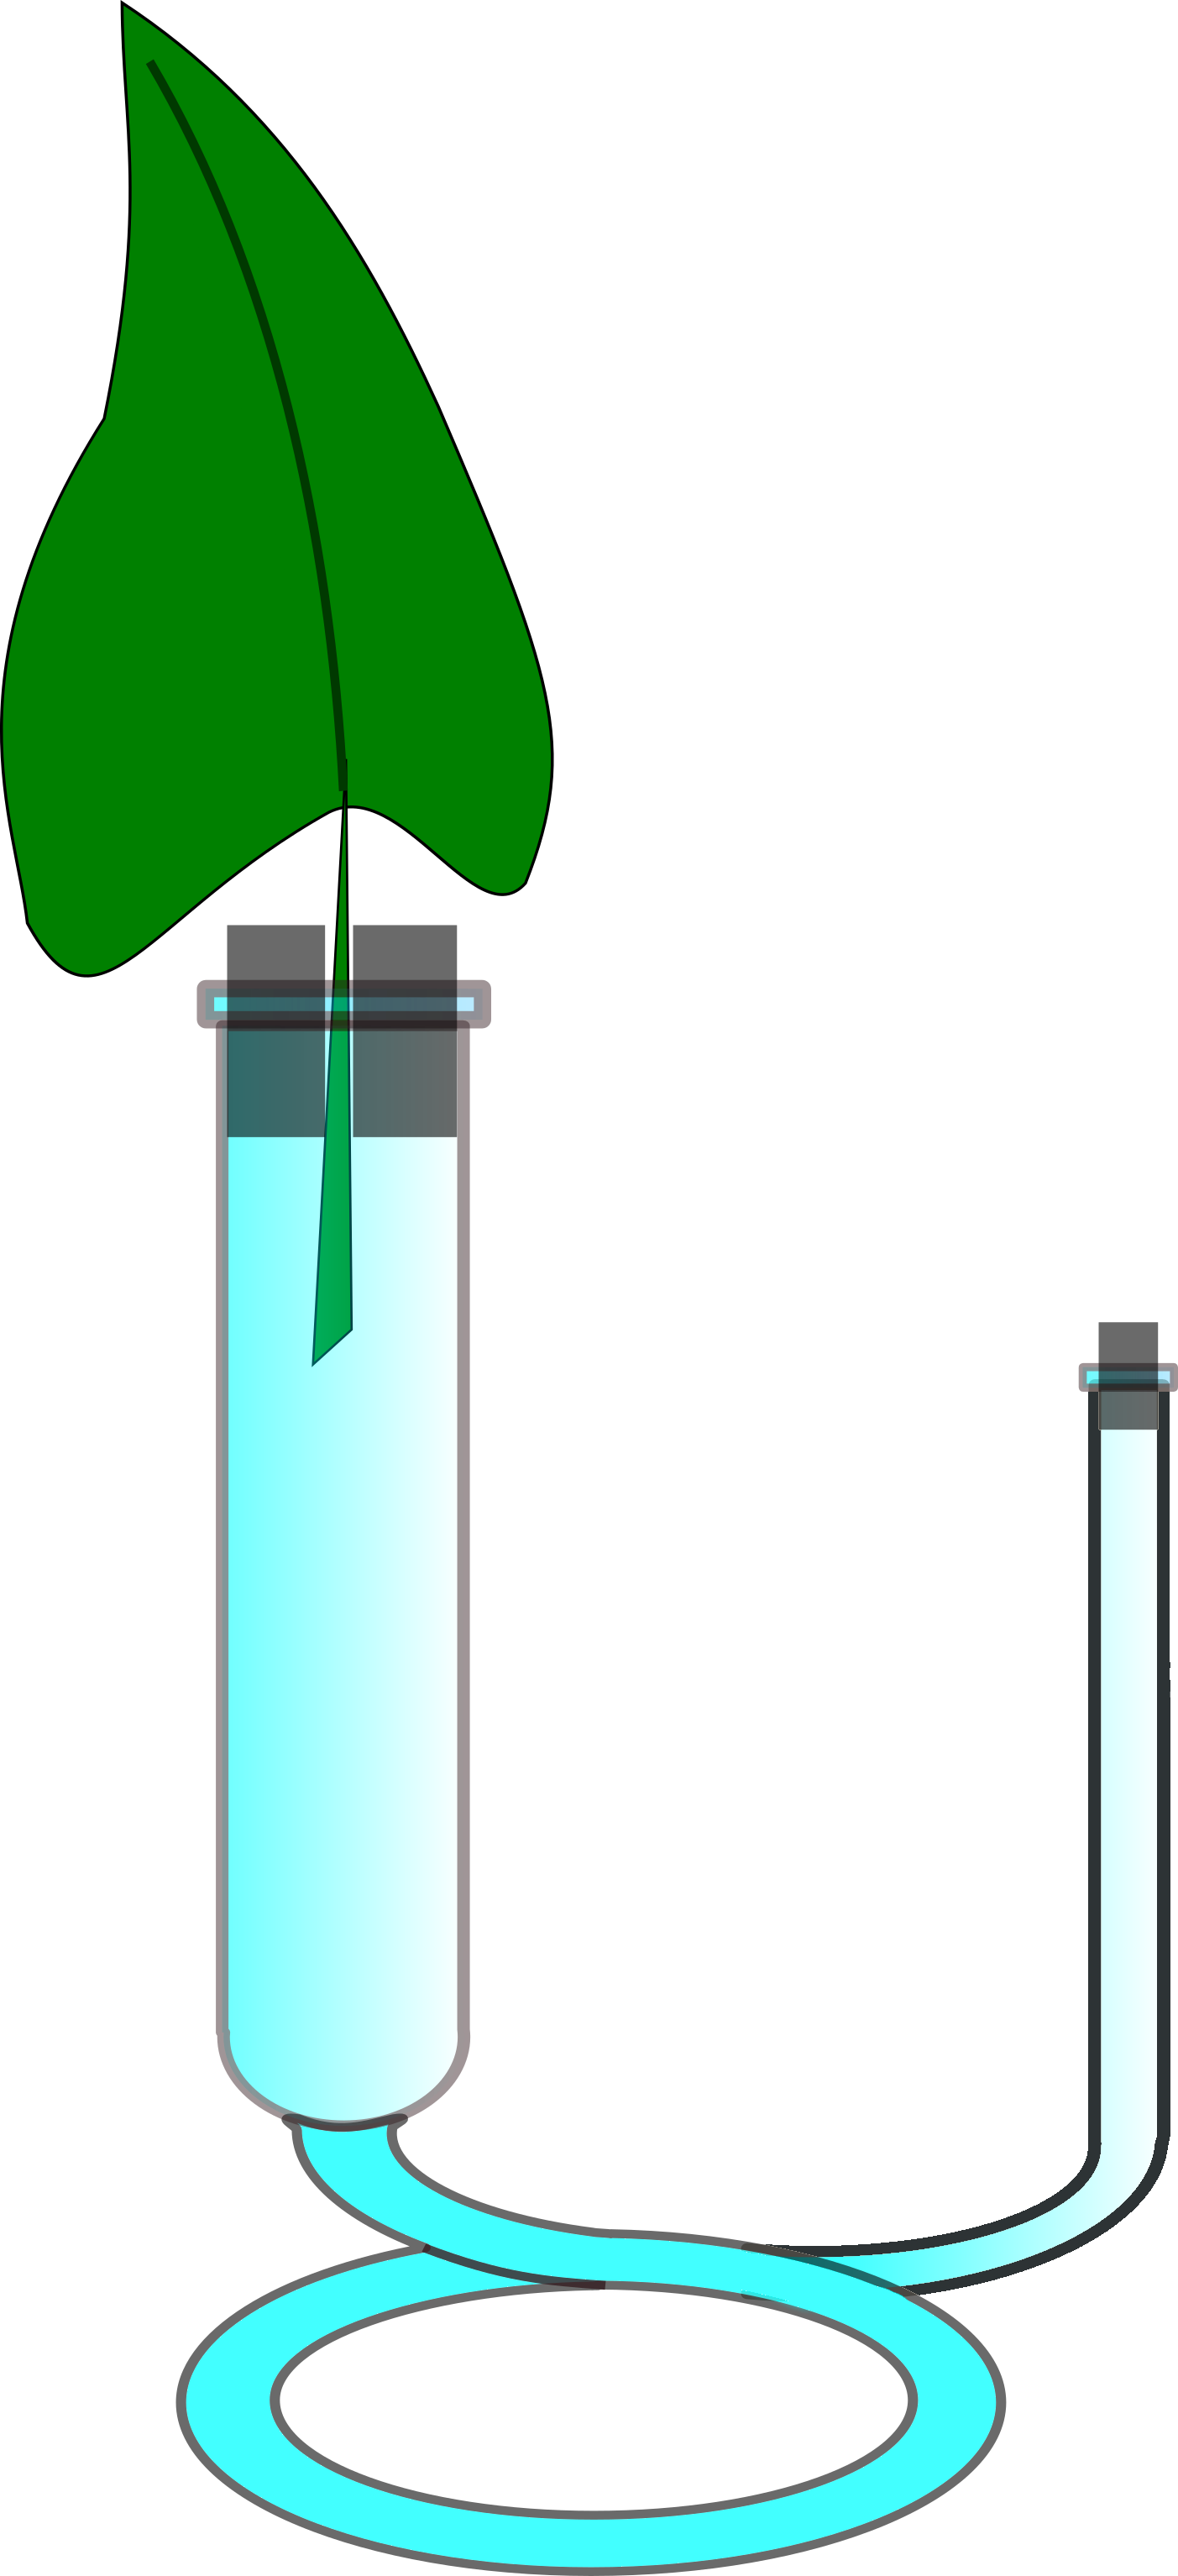
\includegraphics[width=0.2\linewidth]{pictures/veska}
\caption{Прибор Веска в собранном виде}
\label{veska}
\end{figure}
%%%%%%%%%%%%%%%%%%%%%%%%%%%%%%%%%%%%%%%%%%%%%%%%%%%%%%%%%%%%%%%%%%%%%%%%%%%%%%%%%%%%%%%%%%%%%%%%%%%%%%%%%%%

\paragraph*{}Для обеспечения точности измерения, смонтированный и готовый к работе прибор Веска должен быть совершенно сухим, плотно закрытым, пробка не должна касаться воды.

\paragraph*{}Описанным выше образом необходимо приготовить два прибора Веска. Перед началом опыта, приборы с закрепленными листьями необходимо взвесить на аналитических весах и снабдить этикетками с указанием веса прибора. Один из приборов помещается под прямой солнечный свет, например на окно лаборатории, а другой в \hyperlink{light_dark_diferences}{темную камеру}. 

\paragraph*{}Через 1 час после начала опыта взвести приборы повторно. По разнице с первоначальной массой установите количество воды, которое испарил лист за время опыта.

\subsubsection*{Измерение площади листа}

\paragraph*{}Для того, чтобы выполнить расчеты интенсивности транспирации, необходимо знать площадь листа. Площадь листа измеряется следующим способом: из бумаги вырезается квадрат со стороной 10 см. Таким образом, площадь этого квадрата будет составлять 100 см$^2$. Приготовленный для опыта лист необходимо приложить к бумаге, обвести карандашом и вырезать по полученному контуру. 

\paragraph*{}Затем на аналитических весах определите массу квадрата и бумажного контура листа. Площадь листа определяется по пропорции \ref{liaf_square}: 

\begin{equation}
  \label{liaf_square}
  S_l = \frac{S_{sq} * m_l}
                 {m_{sq}}
\end{equation}

\paragraph*{}Где $S_{l}$ – площадь листа, $S_{sq}$ – площадь бумажного квадрата, $m_l$ – масса бумажного контура листа, $m_{sq}$ – масса квадрата.

\subsubsection*{Вычисление интенсивности транспирации}

\paragraph*{}На основании полученных результатов рассчитайте интенсивность транспирации, то есть количество воды в граммах, которое испаряет единица листовой поверхности (1м$^2$) в единицу времени (1 ч).

\paragraph*{}Интенсивность транспирации рассчитывается  по следующей формуле \ref{transpiration_level} 

\begin{equation}
	\label{transpiration_level}
	T = \frac{10000*C}{St}
\end{equation}

\paragraph*{}Где \textit{T} - интенсивность транспирации, \textit{C} - убыль массы листа за время опыта; \textit{S} - площадь листа (м$^2$); \textit{t} - время опыта (ч)

\paragraph*{}\textbf{Сделайте вывод} о том, как сильно отличается уровень транспирации у растения в темноте и на свету. На основе знания о механизме работы устьиц \cite{fzr_ermakov, fzr_jakushina} обоснуйте почему.

\subsection*{Вопросы для самоконтроля}

	\begin{itemize}
		\item Опишите строение клеток \hypertarget{xsilema_tisue}{ксилемы и флоэмы}. Благодаря каким особенностям строения клетки этих тканей приспособлены к транспорту воды?
		\item Из каких компонентов складывается водный режим растения?
		\item Что такое \hypertarget{transpiration_question}{транспирация}? В чем заключается значение транспирации для растения?
		\item От каких факторов зависит \hypertarget{transpiration_intensivity}{интенсивность транспирации}?
		\item \hypertarget{transpiration_air_humidity}{Почему} интенсивность транспирации снижается при повышении относительной влажности воздуха?
		\item Почему сильный ветер способствует более интенсивной транспирации?
		\item \hypertarget{transpiration_time}{В какое время суток} интенсивность транспирации наибольшая. Почему?
		\item Опишите механизм работы устьиц;
		\item Каким образом растения-ксерофиты уменьшают потерю влаги через устьица?
		\item \hypertarget{light_dark_diferences}{Есть} ли различия в интенсивности транспирации побегов на свету и в темноте? Как можно объяснить результаты опыта?
		\item Что такое вещества-антитранспиранты? какие группы антитранспирантов вы знаете;
	\end{itemize}